% !TeX root=../main.tex
\chapter{آشنایی با ابزار‌های توسعه}
در تمام ابزارهای ذکر شده در ادامه این متن حتما باید به ورژن هر کدام دقت شود، ورژن‌ها باید با یکدیگر همخوانی داشته باشند در غیر این صورت مشکلاتی در کامپایل و اجرای برنامه به وجود می‌آید که به راحتی قابل رفع کردن نیستند. در انجام این پروژه عدم همخوانی ورژن‌های مختلف ابزارها با یکدیگر باعث ایجاد مشکلات فراوانی شد، به همین دلیل ورژن مورد نیاز هر ابزار در توضیحات پروژه ذکر شده است.

% ------------ Section 3.1
\section{ابزارهای ساده}
\begin{itemize}
	\item \textbf{ویرایشگر}\\
	برای برنامه نویسی این قرارداد هوشمند از ویرایشگر VSCode با نصب
	پلاگین مربوط به Solidity
\LTRfootnote{https://marketplace.visualstudio.com/items?itemName=JuanBlanco.solidity}
استفاده شده است. این پلاگین با یافتن اشتباه‌ها پیش از کامپایل و راهنمایی در نوشتن کد قرارداد کمک شایانی به افزایش سرعت توسعه می‌کند.

	\item \textbf{ورژن‌کنترل}\\
	این پروژه از روز نخست به صورت متن‌باز توسعه یافته، برای توسعه یک پروژه به صورت متن‌باز اولین ابزار مورد نیاز یک برنامه ورژن کنترل است که نسخه‌های متفاوت و تغییر یافته کدها را به صورت مرتب نگهداری کند. برای این منظور از گیت‌هاب استفاده شده.

	\item \textbf{پکیج‌های Node و NPM}\\
از آنجایی که کدهای سالیدیتی در واقع جاوا‌اسکریپت هستند، به ابزارهای توسعه اپلیکیشن‌های جاوااسکریپت برای توسعه سالیدیتی نیاز است. ابزارهایی مانند Node برای کامپایل کردن برنامه‌های جاوااسکریپت و npm که مدیریت پکیج‌های جاوااسکریپتی که نصب می‌شود را به عهده دارد.

\end{itemize}


% ------------ Section 3.2
\section{کیف پول متامسک}
کیف پول دیجیتال متامسک از پرکاربردترین کیف پول‌ها برای ارتباط برقرار کردن با اپلیکیشن‌های غیرمتمرکز و
\lr{Web3}
است.
کاپو نیز برای امضای تراکنش‌ها و ایجاد ارتباط با شبکه بلاکچین از کیف پول متامسک استفاده می‌کند. برای انجام صحیح این عملیات کاربر باید از پیش کیف پول متامسک را نصب کرده باشد و سپس با انتخاب گزینه
\lr{Connect Wallet}،
کاپو درخواست اتصال به کیف پول و دریافت آدرس کاربر را به متامسک ارسال میکند، متامسک نیز پس از دریافت درخواست کاپو از کاربر اجازه اتصال به اپلیکیشن را میگیرد و در صورت تایید کاربر آدرس کیف پول را به کاپو می‌دهد.

از این پس هرگاه که کابر بخواهد در کاپو تراکنشی از جمله ساخت توکن جدید یا انتقال یک توکن به آدرس دیگر را انجام دهد کاپو از متامسک درخواست می‌کند که با
\gls{Private key}
کاربر آن تراکنش را امضا کند، متامسک از کاربر تایید تراکنش را میگیرد و امضا را انجام می‌دهد و تراکنش به شبکه بلاکچین ارسال می‌شود.


% ------------ Section 3.3
\section{فریمورک‌ها و کتابخانه‌ها}
به دلیل تازگی بحث توسعه اپلیکیشن‌های غیرمتمرکز ابزارهای کمی در این زمینه وجود دارند و همین ابزارها هم معمولا مشکلاتی دارند و به بلوغ کامل نرسیده‌اند. اما با توجه به این که اکثر ابزارها و فریمورک‌ها و کتابخانه‌های توسعه اپلیکیشن‌های غیرمتمرکز متن‌باز هستند، سرعت رشد و تکامل بالایی دارند و به کمک
\glspl{Developer}
این حوزه، هر روز نسبت به روز گذشته پیشرفت می‌کنند.

برای توسعه این پروژه از
فریمورک Truffle
\LTRfootnote{https://trufflesuite.com}،
کتابخانه‌ی OpenZeppelin
\LTRfootnote{https://openzeppelin.com/contracts}،
کتابخانه‌ی
\lr{Web3JS}
\LTRfootnote{https://github.com/ChainSafe/web3.js}
استفاده شده است. در این قسمت به توضیح هر یک از این موارد پرداخته می‌شود.

\subsection{فریمورک Truffle}
این فریمورک ابزارهای اولیه برای ساخت، کامپایل، تست، دیپلوی و مایگریشن قراردادهای هوشمند به زبان سالیدیتی را فراهم می‌کند. پس از نصب این ابزار با اجرای دستور
\lr{truffle init}
می‌توان یک پروژه جدید ترافل ساخت، همچنین میتوان با استفاده از دستور
\lr{truffle unbox}
از یکی از تمپلیت‌های آماده ترافل استفاده کرد.

\begin{figure}[ht]
\centerline{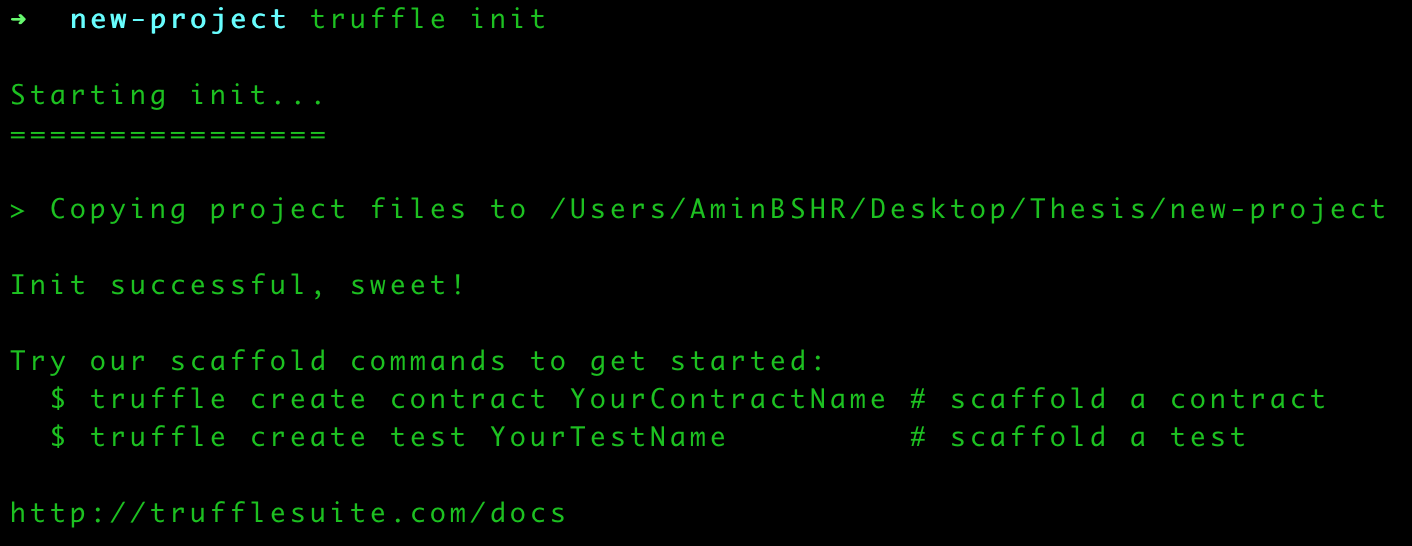
\includegraphics[width=12cm]{truffle-init.png}}
\caption{اجرای دستور \lr{truffle init}}
\label{fig:truffle-init}
\end{figure}

پس از ساخت پروژه با اجرای دستور
\lr{truffle develop}
و یا
\lr{truffle console}
 میتوان وارد خط فرمان ترافل شد.

\begin{figure}[ht]
\centerline{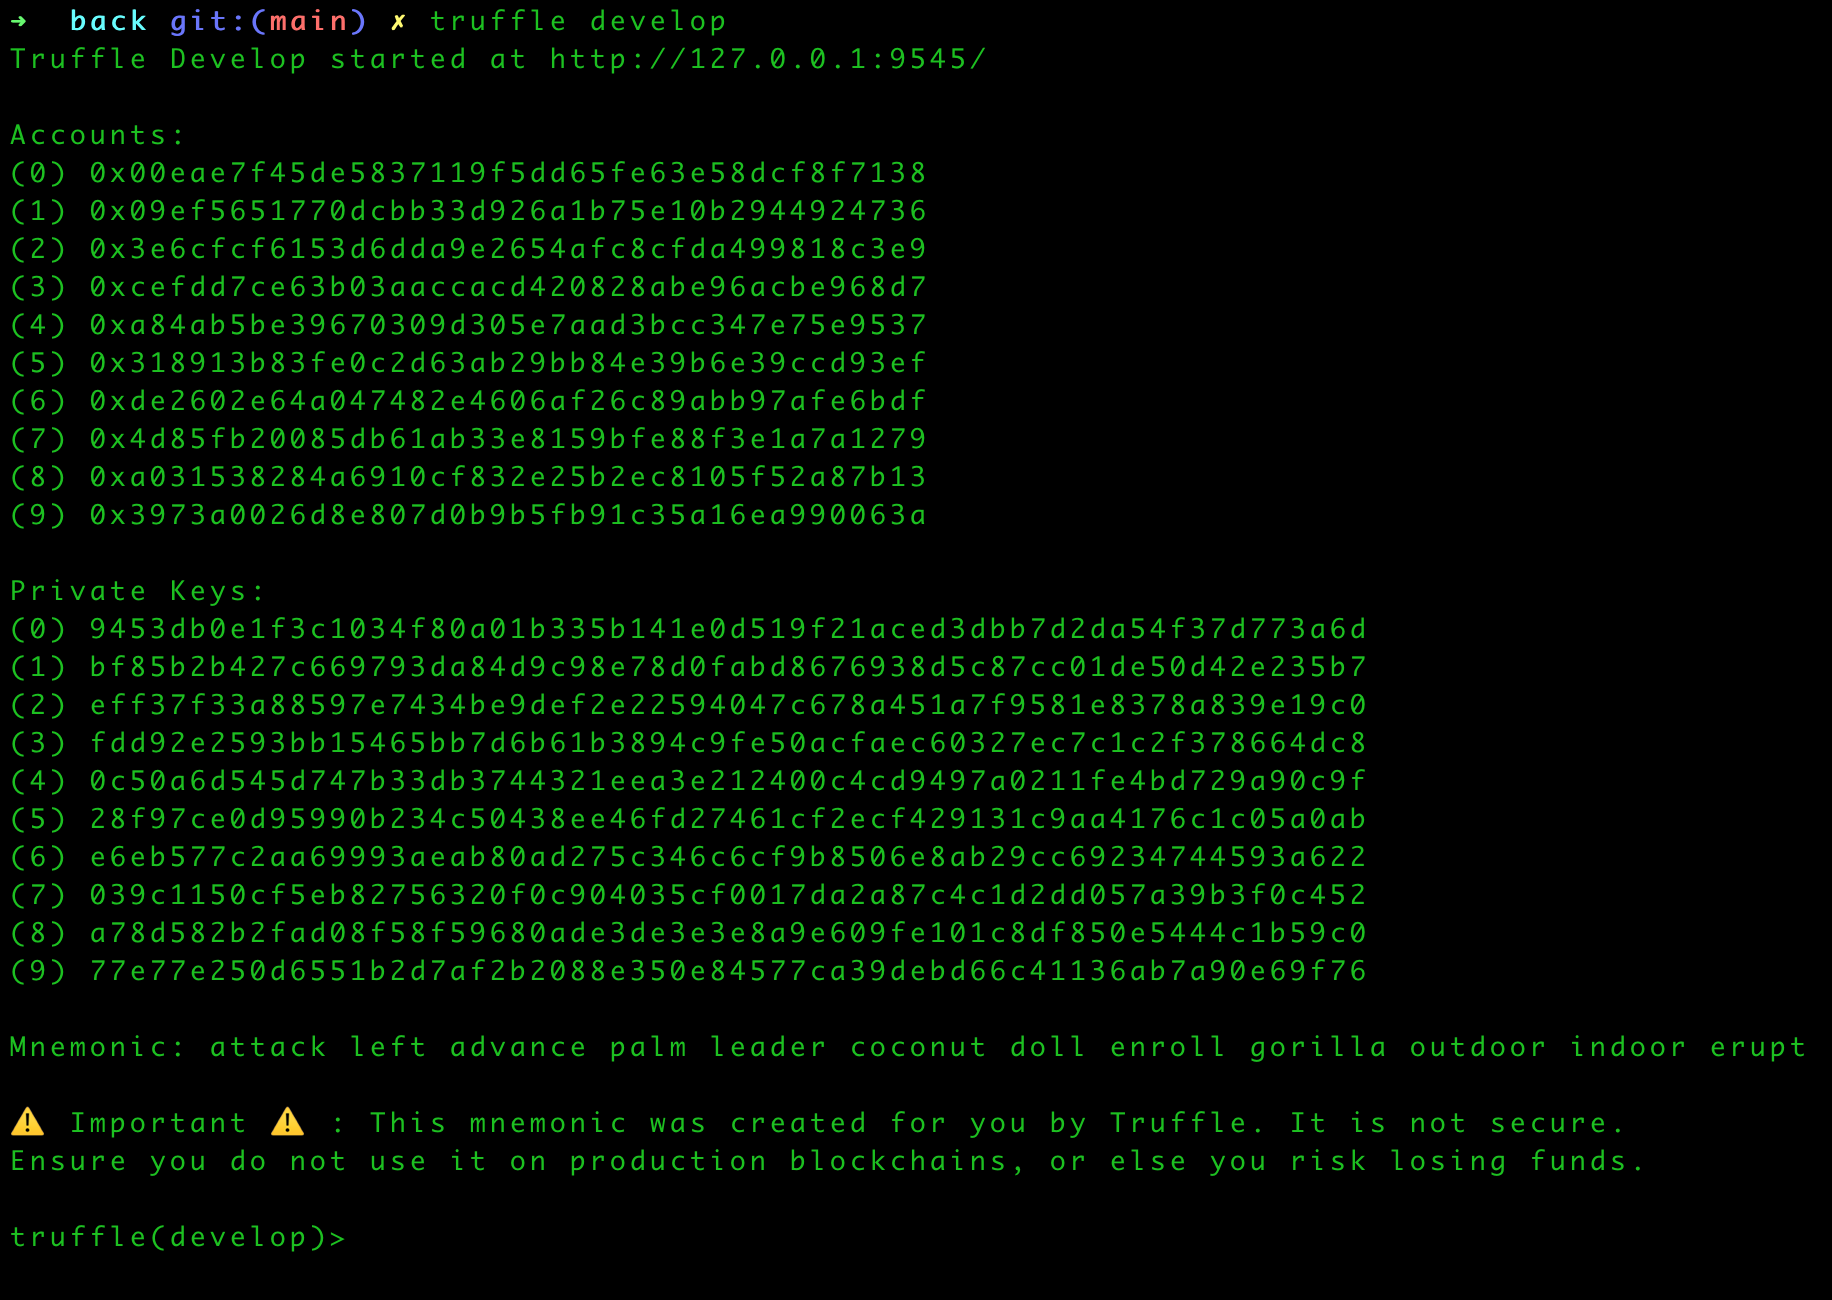
\includegraphics[width=12cm]{truffle-develop.png}}
\caption{اجرای دستور \lr{truffle develop}}
\label{fig:truffle-develop}
\end{figure}

دستورات لازم برای اجرای تست‌ها، کامپیایل کردن قراردادهوشمند یا دیپلوی آن روی شبکه مورد نظر از طریق این خط فرمان قابل اجرا هستند. این پلتفرم ابزارهای فراوانی را در اختیار توسعه دهنده قرار می‌دهد که با تعداد بیشتری از آن‌ها در بخش پیاده‌سازی و دیپلوی کاپو آشنا می‌شویم. همچنین از بزرگترین مزایای استفاده از این فریمورک برقراری ارتباط بسیار آسان با ابزارهای دیگر مانند Ganache و Drizzle است.

\subsection{کتابخانه OpenZeppelin}
یکی از معروف‌ترین کتابخانه‌های قراردادهای هوشمند و استانداردهایشان است. قراردادها و استانداردهای موجود در این کتابخانه کاملا تست شده، داکیومنت شده، ایمن و پایه بسیاری از قراردادهای هوشمند بر بستر بلاکچین هستند.
استانداردهای ذکر شده در این متن مانند،
\lr{ERC20}،
\lr{ERC721}،
\lr{ERC1155}
به همراه تعداد زیادی استانداردهای دیگر در این کتابخانه پیاده‌سازی شده‌اند.

در کاپو نیز از استاندارد
\lr{ERC721}
پیاده‌سازی شده در این کتابخانه استفاده شده است. برای استفاده از قرارداد‌های اپن‌زپلین در قدم اول باید این کتابخانه به کمک دستور
\lr{npm install @openzeppelin/contracts}
نصب شود. پس از نصب کتابخانه، می‌توان از قراردادهای آن ارث‌بری کرد، در قطعه کد زیر مشاهده می‌شود که کاپو چگونه از قرارداد
\lr{ERC721}
موجود در اپن‌زپلین و همچنین یک قراردادهوشمند به اسم Helper که در همین پروژه نوشته شده ارث‌بری کرده است.

\begin{figure}[ht]
\centerline{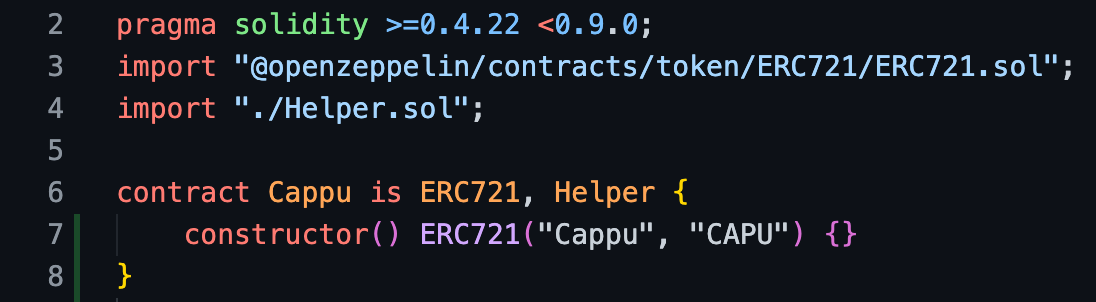
\includegraphics[width=12cm]{inherit-erc721.png}}
\caption{ارث‌بری از استاندارد \lr{ERC721} پیاده‌سازی شده توسط OpenZeppelin}
\label{fig:inherit-erc721}
\end{figure}

\subsection{کتابخانه \lr{Web3JS}}
تراکنش‌های با یک قرارداد هوشمند می‌تواند به ۲ حالت باشد. در حالت اول فقط اطلاعات شبکه بلاکچین خوانده می‌شود و
\gls{State}
آن تغییری داده نمی‌شود، متدهای از این جنس از نوع view یا pure هستند. حالت دوم تراکنش‌هایی هستند که باعث تغییر اطلاعات شبکه بلاکچین می‌شوند.

فرانت‌اند یک اپلیکیشن غیرمتمرکز برای انجام نوع اول تراکنش‌های نهایتا فقط به آدرس کاربر نیاز دارد که اطلاعات مربوط به او را از قرار داد بگیرد. در حالت دوم نیاز است که تراکنشی بر روی شبکه ثبت شود که نیازمند امضا شدن تراکنش توسط کلید خصوصی کاربر، پرداخت کارمزد تراکنش و ارسال آن به نودهای شبکه است.

کتابخانه‌ی
\lr{Web3JS}
به توسعه دهنده کمک می‌کند که فرانت‌اند اپلیکیشن را به کیف پول دیجیتال کاربر و شبکه بلاکچین متصل کند. با ایجاد این اتصال آدرس کابر توسط کیف پول دیجیتال در اختیار فرانت‌اند قرار می‌گیرد و هرگاه که فرانت‌اند بخواهد تراکنشی را روی شبکه ارسال کند نیز از کیف پول کاربر می‌خواهد که با داشتن کلید خصوصی کاربر آن تراکنش را امضا و روی شبکه ارسال کند. طبیعتا کیف پول کاربر برای انجام هر یک از این مراحل از کاربر درخواست تاییدیه می کند.


% ------------ Section 3.4
